\section{Fase C: convergencia dentro de cada camino y entre caminos}
\label{sec:convergencia}

\subsection{Dos preguntas distintas}

Una cadena de Metropolis converge cuando la distribución de su estado ya no depende del punto de partida. Con 100 caminos independientes, esa propiedad se examina de dos maneras complementarias. Dentro de un camino, la serie medida debe ser estacionaria: su media no debe derivar entre el comienzo y el final de la medición. Entre caminos, todas las copias deben describir la misma distribución, porque todas parten de configuraciones distintas pero apuntan a la misma $\pi_\beta$. Una serie puede mostrar estabilidad local mientras permanece en un sector de energía. La comparación entre caminos puede detectar esa limitación si distintas copias ocupan sectores diferentes.

\textbf{Dentro de cada camino} se usaron tres herramientas. La prueba de \citet{geweke1992} compara la media del primer 10~\% de la serie con la del último 50~\% mediante $z=(\bar x_A-\bar x_B)/(\hat\sigma_A^2/n_A+\hat\sigma_B^2/n_B)^{1/2}$, con varianzas espectrales $\hat\sigma^2=\tauint s^2$. En cada temperatura se cuenta la proporción de copias con $|z|>1.96$ y se contrasta con el 5~\% nominal por una prueba binomial, con corrección de Holm sobre las temperaturas. El truncamiento MSER-5 de \citet{white1997} estima cuántos barridos iniciales siguen contaminados por el transitorio. El tiempo $\tauint$ y el tamaño efectivo $n_{\mathrm{ef}}$ completan el diagnóstico.

\textbf{Entre caminos}, la herramienta central es el factor de reducción de escala de \citet{gelman1992}. Con $m=100$ caminos de $n$ barridos, medias $\bar x_j$ y varianzas internas $s_j^2$,
\begin{equation}
W=\frac1m\sum_{j=1}^m s_j^2,\qquad
\frac{B}{n}=\frac{1}{m-1}\sum_{j=1}^m(\bar x_j-\bar x)^2,\qquad
\Rhat=\sqrt{\frac{\frac{n-1}{n}W+\frac{B}{n}}{W}} .
\label{eq:rhat}
\end{equation}
$W$ mide la variabilidad dentro de los caminos y $B/n$ la variabilidad de sus medias. Si todos los caminos muestrean la misma distribución, $B/n\approx\tauint W/n$ y $\Rhat\to1$ cuando $n$ crece. Si los caminos se quedan en valles distintos, $B/n$ no decrece y $\Rhat$ se estanca por encima de uno. El umbral usual es $\Rhat<1.01$ \citep{vehtari2021}. El veredicto oficial usó la versión normalizada por rangos y plegada de \citet{vehtari2021}, la más exigente; las figuras usan la forma clásica de la ecuación~(\ref{eq:rhat}), que permite separar $E$ de $m$. Se añadió una prueba $\chi^2$ de homogeneidad de las medias de las 100 copias, también con corrección de Holm.

Con estas herramientas, una temperatura \emph{converge} si cumple $\Rhat<1.01$ para $E$ y $m$, no presenta exceso de rechazos de Geweke y su truncamiento MSER-5 no supera 500 barridos. Es \emph{representativa} si además las copias son homogéneas. El criterio denominado \emph{confiable} exige por separado ESS mayor que 400 y jackknife por bloques admisible; no exige cumplir el criterio de convergencia. Esa independencia explica porcentajes de confiabilidad superiores a los de convergencia. Un estado converge solo si todas sus 141 temperaturas lo hacen.

\begin{table}[H]
\centering\small
\caption{Veredicto oficial: porcentaje de las 141 temperaturas que cumplen cada criterio y tramo continuo desde 20~K. Ningún estado converge en toda la escalera.}
\label{tab:veredicto}
\begin{tabular}{lcccccccc}
\toprule
Estado & 1 & 2 & 3 & 4 & 5 & 6 & 7 & 8\\
\midrule
Converge (\%) & 30 & 31 & 38 & 54 & 55 & 30 & 38 & 40\\
Tramo convergido (K) & 15.9 & 15.7 & 14.7 & 13.8 & 13.7 & 15.8 & 15.1 & 14.7\\
Representativa (\%) & 29 & 31 & 38 & 46 & 38 & 28 & 36 & 40\\
Confiable (\%) & 30 & 31 & 38 & 72 & 100 & 32 & 40 & 41\\
\bottomrule
\end{tabular}
\end{table}

La tabla~\ref{tab:veredicto} es concluyente en lo global: ningún estado converge en toda la escalera. El mejor caso, $\kdm=1$, cumple en el 55~\% de las temperaturas, sin interrupción de 20.0 a 13.7~K. Por debajo de ese tramo, los resultados no pueden tomarse como muestras de la distribución de equilibrio.

\subsection{Qué converge y qué no: energía frente a magnetización}

La figura~\ref{fig:rhat} separa el diagnóstico por variable y aclara el veredicto. Para la energía, $\Rhat-1$ queda por debajo de 0.01 en todas las temperaturas de siete estados y en el 93~\% de las del estado 5, con un máximo de 1.017. La magnetización se comporta distinto: $\Rhat$ sube de forma sostenida al enfriar, cruza el umbral entre 15.5 y 9.5~K según el estado y alcanza 2.8 a 6~K. El veredicto negativo se debe a $m$, no a $E$.

\begin{figure}[H]
\centering
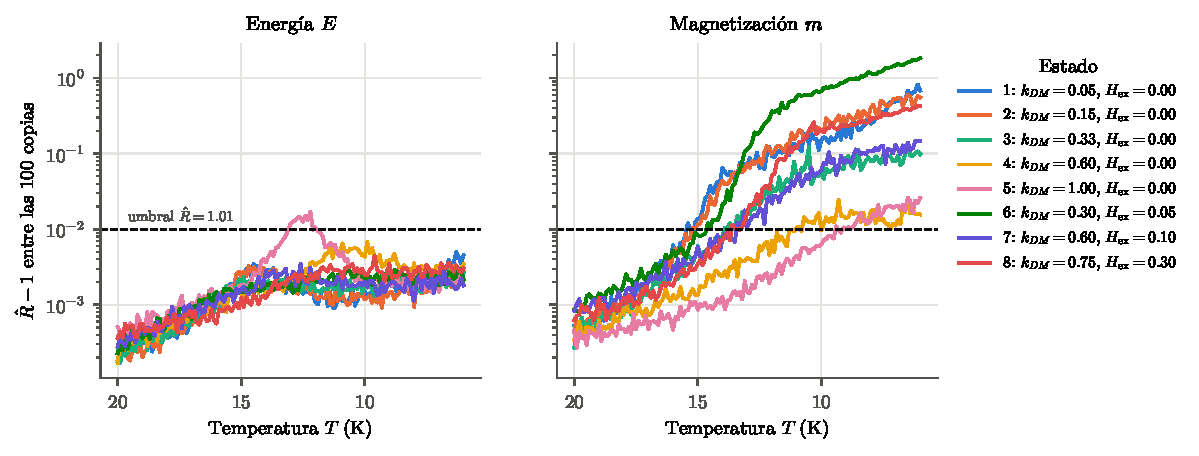
\includegraphics[width=0.92\textwidth]{rhat_T.pdf}
\caption{$\Rhat-1$ entre las 100 copias en cada temperatura, en escala logarítmica. La línea discontinua es el umbral $\Rhat=1.01$; el eje de temperatura avanza en el sentido del enfriamiento.}
\label{fig:rhat}
\end{figure}

\begin{figure}[H]
\centering
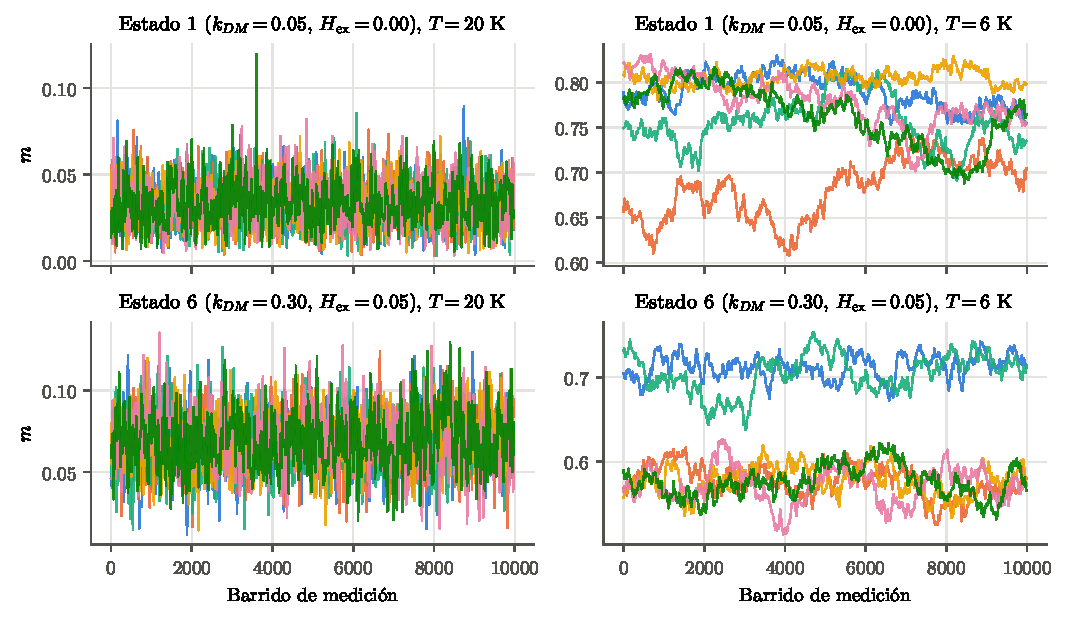
\includegraphics[width=0.88\textwidth]{trazas_m.pdf}
\caption{Magnetización de seis copias durante los 10\,000 barridos de medición (una muestra cada 20 barridos). A 20~K los caminos son indistinguibles; a 6~K cada camino es estable alrededor de su propio nivel y los niveles difieren entre caminos.}
\label{fig:trazas}
\end{figure}

La figura~\ref{fig:trazas} muestra el mecanismo. A 20~K las seis trayectorias se superponen: no se observan diferencias persistentes en esas trazas, de acuerdo con los diagnósticos a esa temperatura. A 6~K cada trayectoria es aproximadamente estacionaria, de modo que el diagnóstico dentro del camino es favorable, pero cada una oscila alrededor de un nivel distinto. En el estado 6 las copias se separan en dos grupos, cerca de $m=0.58$ y $m=0.70$. Así se resuelve la aparente paradoja: dentro de un mismo camino la medición se mantiene igual, como debe ocurrir; entre caminos, la orientación de la textura difiere. Las diferencias de $m$ requieren cambios de alineación relativa, cancelación entre dominios o textura: una rotación rígida conserva la norma de magnetización. Configuraciones con distinta $m$ pueden tener energías próximas. Esa posibilidad explica la diferencia entre diagnósticos, pero la estabilidad de $E$ sola no garantiza la de su varianza. La auditoría adicional examina la fluctuación energética cuadrática cerca del pico.

\subsection{Cuántos pasos Monte Carlo hacen falta}

La pregunta práctica es cuántos barridos adicionales llevarían a $\Rhat<1.01$. Para responderla se recalculó $\Rhat$ con los primeros $n$ barridos de medición, para 25 valores de $n$ entre 100 y 10\,000 (figura~\ref{fig:rhatn}). Si los caminos exploran la misma distribución, $B/n$ decae como $1/n$ y la pendiente de $\log(\Rhat-1)$ frente a $\log n$ es cercana a $-1$. Una pendiente mucho menor en valor absoluto indica caminos atrapados.

\begin{figure}[H]
\centering
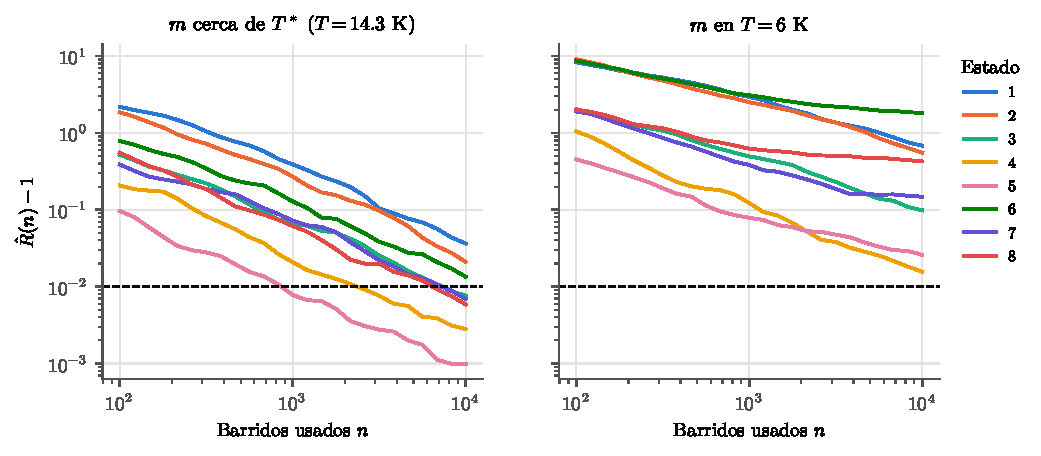
\includegraphics[width=0.88\textwidth]{rhat_n.pdf}
\caption{$\Rhat(n)-1$ de la magnetización calculado con los primeros $n$ barridos de medición, cerca de $T^*$ (izquierda) y a 6~K (derecha). La línea discontinua es el umbral.}
\label{fig:rhatn}
\end{figure}

\begin{figure}[H]
\centering
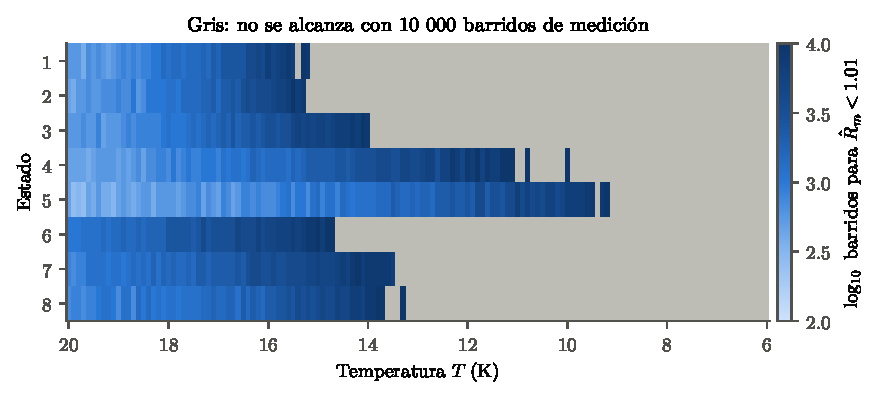
\includegraphics[width=0.92\textwidth]{barridos_necesarios.pdf}
\caption{Barridos de medición necesarios para que $\Rhat_m$ quede por debajo de 1.01 y no vuelva a superarlo, por estado y temperatura. En gris, temperaturas donde 10\,000 barridos no bastan.}
\label{fig:barridos}
\end{figure}

Cerca de $T^*$ la pendiente vale entre $-0.88$ y $-1.08$ en los ocho estados: el régimen es de mezcla lenta pero sana, y la extrapolación orienta hacia $10^4$ a $3.4\times10^4$ barridos. Es una proyección desde la ventana observada y necesita validación mediante corridas más largas. A 6~K aparecen dos comportamientos. En los estados sin campo, la pendiente se mantiene entre $-0.48$ y $-0.87$, y la extrapolación da $1.6\times10^4$ barridos para $\kdm=0.6$, $2.1\times10^5$ para $\kdm=0.33$ y de $4\times10^6$ a $8\times10^6$ para $\kdm\le0.15$, es decir, de 400 a 800 veces el presupuesto usado. Con campo, la pendiente se aplana: $-0.43$ en el estado 7, que necesitaría $3.5\times10^6$ barridos, y $-0.22$ y $-0.15$ en los estados 6 y 8. En estos dos últimos, $\Rhat$ prácticamente no baja con más barridos, y la extrapolación supera los $10^{13}$, una cifra sin utilidad predictiva a esa distancia de los datos. La pendiente observada advierte que debe compararse otro esquema de muestreo antes de invertir en cadenas mucho más largas. La figura~\ref{fig:barridos} resume el mapa completo; el límite entre azul y gris es la temperatura a la que el presupuesto se agotó.

\subsection{Relación con la interacción quiral y el campo}

\begin{table}[H]
\centering\small
\caption{Correlación de Spearman entre los parámetros y las métricas de convergencia de $m$, sobre los ocho estados. IC bootstrap percentil del 95~\% remuestreando estados ($B=20\,000$) y valor $p$ de la prueba de permutación exacta ($8!=40\,320$ asignaciones).}
\label{tab:spearman}
\begin{tabular}{llccc}
\toprule
Métrica & Parámetro & $\rho$ & IC 95~\% & $p$\\
\midrule
fracción de T con $\hat R_m<1.01$ & $k_{DM}$ & $+0.92$ & $[+0.47,\,+1.00]$ & 0.003 \\
fracción de T con $\hat R_m<1.01$ & $H$ & $+0.11$ & $[-0.60,\,+0.84]$ & 0.801 \\
T más baja del tramo convergido en $m$ (K) & $k_{DM}$ & $-0.92$ & $[-1.00,\,-0.47]$ & 0.002 \\
T más baja del tramo convergido en $m$ (K) & $H$ & $-0.11$ & $[-0.81,\,+0.59]$ & 0.827 \\
$\tau_{int}$ máximo de $m$ (barridos) & $k_{DM}$ & $-0.96$ & $[-1.00,\,-0.64]$ & 0.001 \\
$\tau_{int}$ máximo de $m$ (barridos) & $H$ & $-0.14$ & $[-0.94,\,+0.55]$ & 0.762 \\
$\tau_{int}$ máximo de $E$ (barridos) & $k_{DM}$ & $-0.20$ & $[-1.00,\,+0.65]$ & 0.631 \\
$\tau_{int}$ máximo de $E$ (barridos) & $H$ & $-0.52$ & $[-0.96,\,+0.18]$ & 0.208 \\
\bottomrule
\end{tabular}
\end{table}

\begin{figure}[H]
\centering
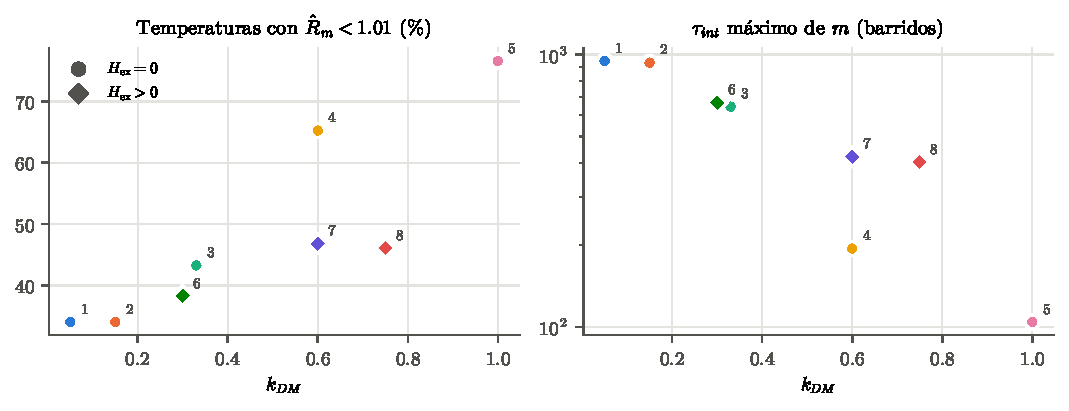
\includegraphics[width=0.9\textwidth]{correlacion_kdm.pdf}
\caption{Fracción de temperaturas convergidas en $m$ (izquierda) y $\tauint$ máximo de $m$ (derecha) frente a $\kdm$. Círculos: $H=0$; rombos: $H>0$; el número identifica el estado.}
\label{fig:corr}
\end{figure}

La interacción quiral gobierna el costo de convergencia de la magnetización (tabla~\ref{tab:spearman} y figura~\ref{fig:corr}). Al pasar de $\kdm=0.05$ a $\kdm=1$, el $\tauint$ máximo de $m$ baja de 946 a 104 barridos ($\rho=-0.96$, $p=0.001$), la fracción de temperaturas convergidas sube del 34 al 77~\% ($\rho=0.92$, $p=0.003$) y el tramo convergido se extiende de 15.5 a 9.5~K. Para la energía no hay relación ($\rho=-0.20$, $p=0.63$). Con solo ocho estados, los intervalos son anchos y la correlación marginal con $H$ no es significativa; además, $H$ y $\kdm$ están confundidos en el diseño, pues los tres estados con campo tienen $\kdm$ intermedio o alto.

Para describir asociaciones condicionadas a ambos parámetros se ajustó por mínimos cuadrados, sobre los $8\times141$ pares (estado, temperatura),
\begin{equation}
\log\tauint(m)=\underset{(0.10)}{3.03}-\underset{(0.07)}{2.37}\,\kdm+\underset{(0.22)}{2.75}\,H+\underset{(0.79)}{30.6}\,\frac1T,\qquad R^2=0.70,
\label{eq:regresion}
\end{equation}
con errores estándar de tipo sándwich (HC0), válidos bajo heterocedasticidad, entre paréntesis. A temperatura fija, aumentar $\kdm$ en 0.1 reduce $\tauint$ en un 21~\% ($e^{-0.237}$), mientras que aumentar $H$ en 0.1 lo multiplica por 1.32. Enfriar de 20 a 6~K lo multiplica por $e^{30.6(1/6-1/20)}\approx35$. Los pares con igual $\kdm$ confirman el signo del campo: con $\kdm=0.6$, $\tauint$ pasa de 194 barridos ($H=0$) a 421 ($H=0.1$). Los errores estándar de la ecuación~(\ref{eq:regresion}) son optimistas, porque temperaturas vecinas de un mismo estado no son independientes; la inferencia sobre los parámetros descansa en la prueba de permutación entre estados. La misma regresión para la energía explica apenas el 24~\% de la variación, con un coeficiente de $\kdm$ de 0.29.

La escala espacial ofrece una explicación plausible para el signo observado de $\kdm$. La espiral tiene período $\lambda=2\pi/\arctan(\kdm/J)$, y el factor de estructura de las configuraciones finales lo confirma: con $\kdm$ de 0.33, 0.6 y 1.0 se miden 18.1, 10.1 y 7.0 sitios, frente a 19.7, 11.6 y 8.0 de la fórmula. Con $\kdm\le0.15$ el período teórico supera los 42 sitios, más que el diámetro del disco (37 sitios), y el período medido se satura en 30.2. Cuando la espiral no cabe en el disco, la textura es casi un único dominio con magnetización neta grande, y su orientación solo cambia rotando el disco entero, un movimiento colectivo que Metropolis, espín por espín, ejecuta con extrema lentitud. Con $\kdm$ grande caben varias vueltas de espiral, la magnetización se promedia entre dominios y cada camino la decorrelaciona pronto. El campo perpendicular, por su parte, estabiliza skyrmiones: a 6~K la carga topológica modal es $Q=0$ en los estados sin campo y $Q=-1$, $-4$ y $-6$ en los estados 6, 7 y 8. Cambiar la categoría de $Q$ puede requerir reorganizaciones difíciles con movimientos locales. Las configuraciones finales y el estancamiento del diagnóstico son compatibles con mezcla limitada, pero no se guardó la trayectoria de $Q$ por barrido para medir tasas de cambio de sector o demostrar que nunca ocurre.

\subsection{Poblaciones ocultas de estados finales: mezclas y algoritmo EM}

Si los caminos terminan en valles distintos, las medias $\bar m_j$ de las 100 copias a 6~K deben provenir de una mezcla de poblaciones. Se ajustaron mezclas gaussianas de $k=1$, 2 y 3 componentes con el algoritmo EM \citep{dempster1977}, programado sin librerías de mezclas. El paso E calcula las responsabilidades $r_{jc}=w_c\,\phi(\bar m_j;\mu_c,\sigma_c^2)/\sum_\ell w_\ell\,\phi(\bar m_j;\mu_\ell,\sigma_\ell^2)$; el paso M actualiza $w_c=\sum_jr_{jc}/100$, $\mu_c$ y $\sigma_c^2$ como medias y varianzas ponderadas. Para cada $k$ se usaron 20 arranques aleatorios, se conservó el de mayor verosimilitud y se eligió $k$ con $\mathrm{BIC}=-2\ell+(3k-1)\log100$ \citep{schwarz1978}. En los 480 ajustes la log-verosimilitud nunca decreció entre iteraciones, como garantiza la teoría del algoritmo.

\begin{table}[H]
\centering\small
\caption{Mezclas gaussianas ajustadas por EM a las medias $\bar m_j$ de las 100 copias a 6~K. Se elige el $k$ de menor BIC; la última columna muestra los pesos y las componentes del modelo elegido.}
\label{tab:em}
\footnotesize\setlength{\tabcolsep}{4pt}
\begin{tabular}{cccccp{8.2cm}}
\toprule
Estado & BIC $k=1$ & BIC $k=2$ & BIC $k=3$ & $k$ & Componentes\\
\midrule
1 & -380.4 & -411.8 & -405.2 & 2 & 0.72\,$\mathcal N(0.775,\,0.015^2)$; 0.28\,$\mathcal N(0.714,\,0.033^2)$ \\
2 & -290.0 & -280.5 & -271.4 & 1 & 1.00\,$\mathcal N(0.300,\,0.054^2)$ \\
3 & -634.0 & -622.9 & -611.5 & 1 & 1.00\,$\mathcal N(0.065,\,0.010^2)$ \\
4 & -959.6 & -948.9 & -943.6 & 1 & 1.00\,$\mathcal N(0.027,\,0.002^2)$ \\
5 & -1004.8 & -1014.8 & -1011.0 & 2 & 0.60\,$\mathcal N(0.015,\,0.001^2)$; 0.40\,$\mathcal N(0.017,\,0.001^2)$ \\
6 & -300.9 & -589.3 & -582.6 & 2 & 0.78\,$\mathcal N(0.580,\,0.007^2)$; 0.22\,$\mathcal N(0.702,\,0.006^2)$ \\
7 & -675.3 & -726.1 & -718.8 & 2 & 0.82\,$\mathcal N(0.389,\,0.003^2)$; 0.18\,$\mathcal N(0.372,\,0.008^2)$ \\
8 & -619.1 & -669.3 & -720.9 & 3 & 0.50\,$\mathcal N(0.577,\,0.003^2)$; 0.39\,$\mathcal N(0.563,\,0.002^2)$; 0.11\,$\mathcal N(0.595,\,0.002^2)$ \\
\bottomrule
\end{tabular}
\end{table}

\begin{figure}[H]
\centering
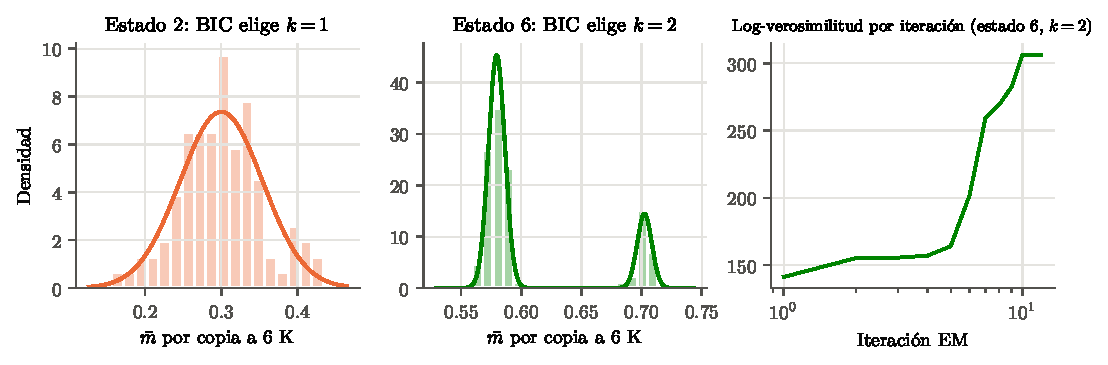
\includegraphics[width=0.95\textwidth]{mezcla_em.pdf}
\caption{Histograma de $\bar m_j$ a 6~K con la mezcla elegida por BIC para los estados 2 y 6, y log-verosimilitud por iteración del mejor arranque del estado 6 con $k=2$.}
\label{fig:em}
\end{figure}

El BIC distingue dos situaciones (tabla~\ref{tab:em} y figura~\ref{fig:em}). En los estados 2, 3 y 4 basta una normal: una sola población estadística describe las medias de $m$ entre las opciones probadas; ello no identifica un único valle físico. En los estados 1, 6 y 8 hay poblaciones separadas. El caso más nítido es el estado 6: el 78~\% de los caminos termina cerca de $m=0.58$ y el 22~\% cerca de $m=0.70$, con desviaciones internas de 0.007, de modo que los grupos no se solapan. La proporción dominante coincide con la del agrupamiento jerárquico del factor de estructura (78~\%). Esa igualdad apoya una comparación entre clasificaciones, pero no demuestra correspondencia individual sin cruzar las etiquetas de cada camino. En el estado 8 el BIC elige tres componentes y la mitad de los caminos comparte la carga modal $Q=-6$. En los estados 5 y 7 las componentes tienen casi la misma media y difieren sobre todo en dispersión; allí la mezcla describe diferencias estadísticas entre caminos y no basta para identificar valles físicos distintos. Estas poblaciones describen la diversidad del protocolo finito. Las realizaciones son válidas para ese protocolo y algunas ventanas pasan pruebas locales de estabilidad; ello no demuestra estacionariedad global ni pesos de Boltzmann. Los pesos de la mezcla son frecuencias de llegada y sus componentes no equivalen automáticamente a fases termodinámicas.
